\section{Data}

In this section, I will present the dataset used for my research and the steps taken to clean and prepare it for analysis.

The SARC \cite{SARC} dataset contains close to one and a half million textual comments from the Reddit social media platform, labeling each entry as sarcastic or not, with a binary 
labeling system where 1 denotes sarcasm and 0 denotes normal text. One of the primary advantages of this dataset is that the labels are self-annotated by the creators of the comments, 
following an established convention in online communities where sarcastic remarks are marked with the "/s" tag. This self-annotation process allows for a more accurate representation 
of the labels, as it reflects the intent of the users themselves rather than relying on external interpretations, which can often introduce ambiguity or mislabeling by readers unfamiliar 
with the creator's intent.

In addition to the sarcasm labels and comments, SARC includes a rich variety of metadata associated with every comment, such as the subreddit it was posted in, the parent comment and the 
number of upvotes and downvotes. This metadata enables researchers to analyze the influence of contextual factors on the interpretation of sarcasm. While it is true that sarcasm often 
relies on context, my theory is that most of the times, sarcasm is depicted by repeating certain words or acronyms, which do not have anything to do with the context. This assertion is 
backed up by \cite{Juli_2024}, especially since the majority of online users are younger generations who may use specific slang or phrases that indicate sarcasm independently of the 
surrounding context.

The substantial size of the dataset presents a significant advantage. With over 1 million entries, it offers a valuable resource for training machine learning models. A larger dataset 
generally improves model performance by allowing it to learn from a diverse array of examples. This diversity is especially important for natural language processing tasks, where 
recognizing linguistic nuances and patterns is essential for effective comprehension and prediction.

I began by examining the dataset with the \texttt{info()} function, which revealed the presence of 55 null values in the comments column. I decided to remove these null entries, as null 
data can lead to inaccuracies in model training and evaluation. In addition to the null values, I also identified 28 duplicate entries scattered throughout the dataset. Duplicate data 
can introduce bias, so I opted to eliminate these redundant entries as well.

Following these cleaning operations, I checked the class distribution within the dataset. I found that it remains nearly perfectly balanced, containing 505,403 non-sarcastic comments and 
505,340 sarcastic ones. Figure \ref{Fig_1} illustrates the class distribution following the data cleaning steps.

\begin{figure}
    \centering
    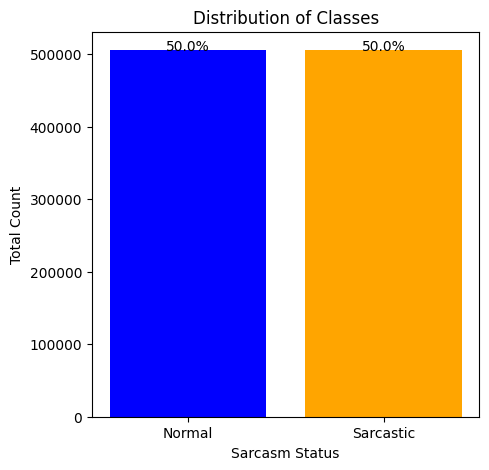
\includegraphics[width=0.5\linewidth]{img/class-dist.png}
    \caption{Class Distribution}
    \label{Fig_1}
\end{figure}

The class distribution plot shows that the dataset is close to perfectly balanced, with both classes appearing in equal proportions. This balanced distribution is a significant advantage 
for model training, as it reduces the risk of bias towards one class over the other. In many real-world classification problems, class imbalance can cause the model to overfit to the 
majority class, making it harder to accurately predict instances of the minority class. However, with an equal split, the model can learn to identify both classes effectively.

From a practical standpoint, this balanced distribution simplifies model evaluation. Metrics such as accuracy, precision, recall, and F1-score will likely give a more reliable indication 
of the model's true performance across both classes. For instance, in an imbalanced scenario, accuracy alone can be misleading if the model simply predicts the majority class most of the 
time. In this case, accuracy is more meaningful, as each class is equally represented. Moreover, the distribution eliminates the need for data augmentation techniques to artificially 
adjust class balance.

For the purpose of this research, I focused on retaining only the labels and comments columns from the dataset, as the other columns did not provide significant contextual value for this 
analysis, as I mentioned earlier.

The next step involved implementing a text preprocessing function to prepare the comments for model evaluation. First, the function converts all letters to lowercase and removes any unnecessary spaces to create a uniform format. 
Afterwards, it addresses contractions using the "contractions" Python library. This process transforms shortened forms of words or combinations of words (e.g., "don't" becomes "do not") 
for better processing.

I also considered lemmatization, which is a process that reduces words to their dictionary form (e.g., "running" becomes "run"). However, I decided against using this technique because 
it negatively impacted model performance. Lemmatization can sometimes eliminate various sarcastic nuances, as certain words can carry different meanings depending on their grammatical form.

Additionally, I removed newline characters to maintain a continuous flow of text. I also inserted spaces to separate words from punctuation marks and replaced any instances of more than 
two consecutive spaces with a single space. This preprocessing function was then applied to the entire comments column.

I also conducted an analysis on comment length distribution, displayed in Figure \ref{Fig_2}, to examine how the lengths of both normal and sarcastic comments are distributed within the 
dataset.

\begin{figure}
    \centering
    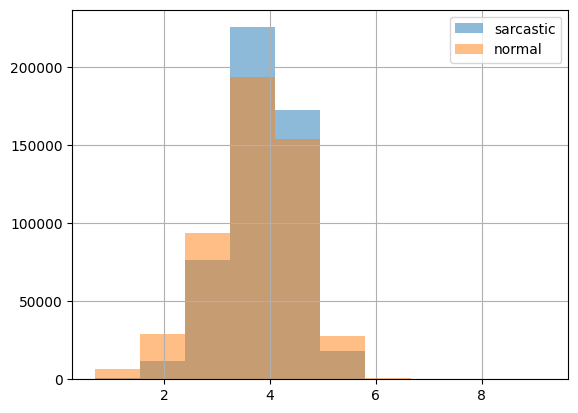
\includegraphics[width=0.5\linewidth]{img/length-dist.png}
    \caption{Comment Length Distribution}
    \label{Fig_2}
\end{figure}

It can be observed that most comments fall within a relatively short length range, with the highest concentration between 3 and 5 words. The peak around this range indicates that both 
normal and sarcastic comments share a similar length distribution, as their overlapping bars show nearly identical trends.

Interestingly, while there are some longer comments in the dataset, their frequency is significantly lower. Beyond a length of 6 words, the number of comments drops off steeply, and 
comments exceeding 8 words appear to be very rare. This suggests that most of the text samples in the dataset are short, reflecting the nature of user-generated comments on social media 
platforms. The near-identical distribution between the two classes also implies that sarcasm in this dataset is not necessarily linked to longer comments, but rather to the choice of 
specific words or acronyms.

The balanced distribution of comment lengths between sarcastic and normal comments ensures that the model will not develop a bias towards identifying sarcasm simply based on comment 
length. This characteristic makes it necessary for the model to rely on deeper linguistic patterns to effectively distinguish between the two classes.
